%!TEX program = xelatex 
%!TEX encoding = ISO-8859-1
%%%%%%%%%%%%%%%%%%%%%%%%%%%%%%%%%%%%%%%%%
% The Legrand Orange Book
% LaTeX Template
% Version 2.3 (8/8/17)
%
% This template has been downloaded from:
% http://www.LaTeXTemplates.com
%
% Original author:
% Mathias Legrand (legrand.mathias@gmail.com) with modifications by:
% Vel (vel@latextemplates.com)
%
% License:
% CC BY-NC-SA 3.0 (http://creativecommons.org/licenses/by-nc-sa/3.0/)
%
% Compiling this template:
% This template uses biber for its bibliography and makeindex for its index.
% When you first open the template, compile it from the command line with the 
% commands below to make sure your LaTeX distribution is configured correctly:
%
% 1) pdflatex main
% 2) makeindex main.idx -s StyleInd.ist
% 3) biber main
% 4) pdflatex main x 2
%
% After this, when you wish to update the bibliography/index use the appropriate
% command above and make sure to compile with pdflatex several times 
% afterwards to propagate your changes to the document.
%
% This template also uses a number of packages which may need to be
% updated to the newest versions for the template to compile. It is strongly
% recommended you update your LaTeX distribution if you have any
% compilation errors.
%
% Important note:
% Chapter heading images should have a 2:1 width:height ratio,
% e.g. 920px width and 460px height.
%
%%%%%%%%%%%%%%%%%%%%%%%%%%%%%%%%%%%%%%%%%

%----------------------------------------------------------------------------------------
%	PACKAGES AND OTHER DOCUMENT CONFIGURATIONS
%----------------------------------------------------------------------------------------

\documentclass[11pt,fleqn]{book} % Default font size and left-justified equations

%----------------------------------------------------------------------------------------

%!TEX program = xelatex
%!TEX root = Algebra_1.tex
%%%%%%%%%%%%%%%%%%%%%%%%%%%%%%%%%%%%%%%%%
% The Legrand Orange Book
% Structural Definitions File
% Version 2.0 (9/2/15)
%
% Original author:
% Mathias Legrand (legrand.mathias@gmail.com) with modifications by:
% Vel (vel@latextemplates.com)
% 
% This file has been downloaded from:
% http://www.LaTeXTemplates.com
%
% License:
% CC BY-NC-SA 3.0 (http://creativecommons.org/licenses/by-nc-sa/3.0/)
%
%%%%%%%%%%%%%%%%%%%%%%%%%%%%%%%%%%%%%%%%%

%----------------------------------------------------------------------------------------
%	VARIOUS REQUIRED PACKAGES AND CONFIGURATIONS
%----------------------------------------------------------------------------------------

\usepackage[top=3cm,bottom=3cm,left=3cm,right=3cm,headsep=10pt,a4paper]{geometry} % Page margins

\usepackage{graphicx} % Required for including pictures
\graphicspath{{Pictures/}} % Specifies the directory where pictures are stored

\usepackage{ccicons} %ícones creative commons

\usepackage{amssymb,amsmath,amsfonts,amsthm,amstext}

\usepackage{enumitem}

\usepackage{lipsum} % Inserts dummy text

\usepackage{tikz} % Required for drawing custom shapes

\usepackage[brazil]{babel}

\usepackage{multicol}

\usepackage{enumitem} % Customize lists
\setlist{nolistsep} % Reduce spacing between bullet points and numbered lists

\usepackage{booktabs} % Required for nicer horizontal rules in tables

\usepackage{xcolor} % Required for specifying colors by name
\definecolor{ocre}{RGB}{243,102,25} % Define the orange color used for highlighting throughout the book

%----------------------------------------------------------------------------------------
%	FONTS
%----------------------------------------------------------------------------------------

\usepackage{avant} % Use the Avantgarde font for headings
%\usepackage{times} % Use the Times font for headings
\usepackage{mathptmx} % Use the Adobe Times Roman as the default text font together with math symbols from the Sym­bol, Chancery and Com­puter Modern fonts

\usepackage{microtype} % Slightly tweak font spacing for aesthetics
\usepackage[utf8]{inputenc} % Required for including letters with accents
\usepackage[T1]{fontenc} % Use 8-bit encoding that has 256 glyphs

%----------------------------------------------------------------------------------------
%	BIBLIOGRAPHY AND INDEX
%----------------------------------------------------------------------------------------

% \usepackage[style=numeric,citestyle=numeric,sorting=nyt,sortcites=true,autopunct=true,babel=hyphen,hyperref=true,abbreviate=false,backref=true,backend=biber]{biblatex}
% \addbibresource{bibliography.bib} % BibTeX bibliography file
% \defbibheading{bibempty}{}

\usepackage{calc} % For simpler calculation - used for spacing the index letter headings correctly
\usepackage{makeidx} % Required to make an index
\makeindex % Tells LaTeX to create the files required for indexing

%----------------------------------------------------------------------------------------
%	MAIN TABLE OF CONTENTS
%----------------------------------------------------------------------------------------

\usepackage{titletoc} % Required for manipulating the table of contents

\contentsmargin{0cm} % Removes the default margin

% Part text styling
\titlecontents{part}[0cm]
{\addvspace{20pt}\centering\large\bfseries}
{}
{}
{}

% Chapter text styling
\titlecontents{chapter}[1.25cm] % Indentation
{\addvspace{12pt}\large\sffamily\bfseries} % Spacing and font options for chapters
{\color{ocre!60}\contentslabel[\Large\thecontentslabel]{1.25cm}\color{ocre}} % Chapter number
{\color{ocre}}  
{\color{ocre!60}\normalsize\;\titlerule*[.5pc]{.}\;\thecontentspage} % Page number

% Section text styling
\titlecontents{section}[1.25cm] % Indentation
{\addvspace{3pt}\sffamily\bfseries} % Spacing and font options for sections
{\contentslabel[\thecontentslabel]{1.25cm}} % Section number
{}
{\hfill\color{black}\thecontentspage} % Page number
[]

% Subsection text styling
\titlecontents{subsection}[1.25cm] % Indentation
{\addvspace{1pt}\sffamily\small} % Spacing and font options for subsections
{\contentslabel[\thecontentslabel]{1.25cm}} % Subsection number
{}
{\ \titlerule*[.5pc]{.}\;\thecontentspage} % Page number
[]

% List of figures
\titlecontents{figure}[0em]
{\addvspace{-5pt}\sffamily}
{\thecontentslabel\hspace*{1em}}
{}
{\ \titlerule*[.5pc]{.}\;\thecontentspage}
[]

% List of tables
\titlecontents{table}[0em]
{\addvspace{-5pt}\sffamily}
{\thecontentslabel\hspace*{1em}}
{}
{\ \titlerule*[.5pc]{.}\;\thecontentspage}
[]

%----------------------------------------------------------------------------------------
%	MINI TABLE OF CONTENTS IN PART HEADS
%----------------------------------------------------------------------------------------

% Chapter text styling
\titlecontents{lchapter}[0em] % Indenting
{\addvspace{15pt}\large\sffamily\bfseries} % Spacing and font options for chapters
{\color{ocre}\contentslabel[\Large\thecontentslabel]{1.25cm}\color{ocre}} % Chapter number
{}  
{\color{ocre}\normalsize\sffamily\bfseries\;\titlerule*[.5pc]{.}\;\thecontentspage} % Page number

% Section text styling
\titlecontents{lsection}[0em] % Indenting
{\sffamily\small} % Spacing and font options for sections
{\contentslabel[\thecontentslabel]{1.25cm}} % Section number
{}
{}

% Subsection text styling
\titlecontents{lsubsection}[.5em] % Indentation
{\normalfont\footnotesize\sffamily} % Font settings
{}
{}
{}

%----------------------------------------------------------------------------------------
%	PAGE HEADERS
%----------------------------------------------------------------------------------------

\usepackage{fancyhdr} % Required for header and footer configuration

\pagestyle{fancy}
\renewcommand{\chaptermark}[1]{\markboth{\sffamily\normalsize\bfseries\chaptername\ \thechapter.\ #1}{}} % Chapter text font settings
\renewcommand{\sectionmark}[1]{\markright{\sffamily\normalsize\thesection\hspace{5pt}#1}{}} % Section text font settings
\fancyhf{} \fancyhead[LE,RO]{\sffamily\normalsize\thepage} % Font setting for the page number in the header
\fancyhead[LO]{\rightmark} % Print the nearest section name on the left side of odd pages
\fancyhead[RE]{\leftmark} % Print the current chapter name on the right side of even pages
\renewcommand{\headrulewidth}{0.5pt} % Width of the rule under the header
\addtolength{\headheight}{2.5pt} % Increase the spacing around the header slightly
\renewcommand{\footrulewidth}{0pt} % Removes the rule in the footer
\fancypagestyle{plain}{\fancyhead{}\renewcommand{\headrulewidth}{0pt}} % Style for when a plain pagestyle is specified

% Removes the header from odd empty pages at the end of chapters
\makeatletter
\renewcommand{\cleardoublepage}{
\clearpage\ifodd\c@page\else
\hbox{}
\vspace*{\fill}
\thispagestyle{empty}
\newpage
\fi}

%----------------------------------------------------------------------------------------
%	THEOREM STYLES
%----------------------------------------------------------------------------------------

\usepackage{amsmath,amsfonts,amssymb,amsthm} % For math equations, theorems, symbols, etc

\newcommand{\intoo}[2]{\mathopen{]}#1\,;#2\mathclose{[}}
\newcommand{\ud}{\mathop{\mathrm{{}d}}\mathopen{}}
\newcommand{\intff}[2]{\mathopen{[}#1\,;#2\mathclose{]}}
\newtheorem{notation}{Notation}[chapter]
\newtheoremstyle{dotless}{}{}{\itshape}{}{\bfseries}{}{ }{}
\theoremstyle{dotless}
\newtheorem*{solucao}{Solu{\c c}{\~a}o:}

% Boxed/framed environments
\newtheoremstyle{ocrenumbox}% % Theorem style name
{0pt}% Space above
{0pt}% Space below
{\normalfont}% % Body font
{}% Indent amount
{\small\bf\sffamily\color{ocre}}% % Theorem head font
{\;}% Punctuation after theorem head
{0.25em}% Space after theorem head
{\small\sffamily\color{ocre}\thmname{#1}\nobreakspace\thmnumber{\@ifnotempty{#1}{}\@upn{#2}}% Theorem text (e.g. Theorem 2.1)
\thmnote{\nobreakspace\the\thm@notefont\sffamily\bfseries\color{black}---\nobreakspace#3.}} % Optional theorem note
\renewcommand{\qedsymbol}{$\blacksquare$}% Optional qed square

\newtheoremstyle{blacknumex}% Theorem style name
{5pt}% Space above
{5pt}% Space below
{\normalfont}% Body font
{} % Indent amount
{\small\bf\sffamily}% Theorem head font
{\;}% Punctuation after theorem head
{0.25em}% Space after theorem head
{\small\sffamily{\tiny\ensuremath{\blacksquare}}\nobreakspace\thmname{#1}\nobreakspace\thmnumber{\@ifnotempty{#1}{}\@upn{#2}}% Theorem text (e.g. Theorem 2.1)
\thmnote{\nobreakspace\the\thm@notefont\sffamily\bfseries---\nobreakspace#3.}}% Optional theorem note

\newtheoremstyle{blacknumbox} % Theorem style name
{0pt}% Space above
{0pt}% Space below
{\normalfont}% Body font
{}% Indent amount
{\small\bf\sffamily}% Theorem head font
{\;}% Punctuation after theorem head
{0.25em}% Space after theorem head
{\small\sffamily\thmname{#1}\nobreakspace\thmnumber{\@ifnotempty{#1}{}\@upn{#2}}% Theorem text (e.g. Theorem 2.1)
\thmnote{\nobreakspace\the\thm@notefont\sffamily\bfseries---\nobreakspace#3.}}% Optional theorem note

% Non-boxed/non-framed environments
\newtheoremstyle{ocrenum}% % Theorem style name
{5pt}% Space above
{5pt}% Space below
{\normalfont}% % Body font
{}% Indent amount
{\small\bf\sffamily\color{ocre}}% % Theorem head font
{\;}% Punctuation after theorem head
{0.25em}% Space after theorem head
{\small\sffamily\color{ocre}\thmname{#1}\nobreakspace\thmnumber{\@ifnotempty{#1}{}\@upn{#2}}% Theorem text (e.g. Theorem 2.1)
\thmnote{\nobreakspace\the\thm@notefont\sffamily\bfseries\color{black}---\nobreakspace#3.}} % Optional theorem note
\renewcommand{\qedsymbol}{$\blacksquare$}% Optional qed square
\makeatother

% Defines the theorem text style for each type of theorem to one of the three styles above
\newcounter{dummy} 
\numberwithin{dummy}{section}
\theoremstyle{ocrenumbox}
\newtheorem{teoremaT}[dummy]{Teorema}
\newtheorem{problema}{Problema}[chapter]
\newtheorem{exercicio}{Exercício}[chapter]
\theoremstyle{blacknumex}
\newtheorem{exemplo}{Exemplo}[chapter]
\newtheorem{exemplos}{Exemplos}[chapter]
\newtheorem{observacao}{Observaçao}[chapter]
\newtheorem{observacoes}{Observações}[chapter]
\newtheorem{nota}{Nota}[chapter]
\theoremstyle{blacknumbox}
\newtheorem{vocabulary}{Vocabulary}[chapter]
\newtheorem{definicaoT}{Definição}[section]
\newtheorem{definicoesT}{Definições}[section]
\newtheorem{corolarioT}[dummy]{Corolário}
\theoremstyle{ocrenum}
\newtheorem{proposicao}[dummy]{Proposição}
\newenvironment{prova}[1][Prova]{\noindent\textbf{#1:} }{\qedsymbol}%{\ \rule{0.5em}{0.5em}}

%----------------------------------------------------------------------------------------
%	MATH COMMANDS
%----------------------------------------------------------------------------------------


\newcommand{\n}{\mathbb{N}}
\newcommand{\z}{\mathbb{Z}}
\newcommand{\rac}{\mathbb{Q}}
\newcommand{\dom}{{\rm dom\,}}
\newcommand{\im}{{\rm Im\,}}
\newcommand{\aut}{{\rm Aut\,}}
\newcommand{\cp}[1]{\mathbb{#1}}
\newcommand{\sub}{\subseteq}
\newcommand{\real}{\mathbb{R}}
\newcommand{\complex}{\mathbb{C}}
\newcommand{\lap}[1]{\mathcal{L}\left\{#1\right\}}
\newcommand{\lapi}[1]{\mathcal{L}^{-1}\left\{#1\right\}}
\newcommand{\se}[1]{\displaystyle\sum_{n = 1}^\infty{#1}}
\newcommand{\dlim}[2]{\displaystyle\lim_{#1\rightarrow #2}}
\newcommand{\slim}{\displaystyle\lim_{n \rightarrow \infty}}
\newcommand{\seq}[1]{\{{#1_n\}}}
\newcommand{\seg}[1]{\displaystyle\sum_{n = 1}^\infty{#1_n}}
\newcommand{\sei}[2]{\displaystyle\sum_{#1}^\infty{#2}}
\newcommand{\sepc}[3]{\displaystyle\sum_{#1}^\infty{#2(x - #3)^n}}
\newcommand{\imp}[3]{\displaystyle\int_{#1}^{+\infty}{#3}{d #2}}
\newcommand{\dint}[4]{\displaystyle\int_{#1}^{#2}{#4}{d#3}}
\newcommand{\inti}[2]{\displaystyle\int{#1}{d#2}}
\newcommand{\norma}[1]{\left\lVert#1\right\rVert}
\newcommand{\flim}[1]{\displaystyle\lim_{#1\rightarrow \infty}}
\renewcommand{\sin}{{\rm sen\,}}
\renewcommand{\tan}{{\rm tg\,}}
\renewcommand{\csc}{{\rm cossec\,}}
\renewcommand{\cot}{{\rm cotg\,}}
\renewcommand{\sinh}{{\rm senh\,}}
\newcommand\T{\rule{0pt}{2.6ex}} 


%----------------------------------------------------------------------------------------
%	DEFINITION OF COLORED BOXES
%----------------------------------------------------------------------------------------

\RequirePackage[framemethod=default]{mdframed} % Required for creating the theorem, definition, exercise and corollary boxes

% Theorem box
\newmdenv[skipabove=7pt,
skipbelow=7pt,
backgroundcolor=black!5,
linecolor=ocre,
innerleftmargin=5pt,
innerrightmargin=5pt,
innertopmargin=5pt,
leftmargin=0cm,
rightmargin=0cm,
innerbottommargin=5pt]{tBox}

% Exercise box	  
\newmdenv[skipabove=7pt,
skipbelow=7pt,
rightline=false,
leftline=true,
topline=false,
bottomline=false,
backgroundcolor=ocre!10,
linecolor=ocre,
innerleftmargin=5pt,
innerrightmargin=5pt,
innertopmargin=5pt,
innerbottommargin=5pt,
leftmargin=0cm,
rightmargin=0cm,
linewidth=4pt]{eBox}	

% Definition box
\newmdenv[skipabove=7pt,
skipbelow=7pt,
rightline=false,
leftline=true,
topline=false,
bottomline=false,
linecolor=ocre,
innerleftmargin=5pt,
innerrightmargin=5pt,
innertopmargin=0pt,
leftmargin=0cm,
rightmargin=0cm,
linewidth=4pt,
innerbottommargin=0pt]{dBox}	

% Corollary box
\newmdenv[skipabove=7pt,
skipbelow=7pt,
rightline=false,
leftline=true,
topline=false,
bottomline=false,
linecolor=gray,
backgroundcolor=black!5,
innerleftmargin=5pt,
innerrightmargin=5pt,
innertopmargin=5pt,
leftmargin=0cm,
rightmargin=0cm,
linewidth=4pt,
innerbottommargin=5pt]{cBox}

% Creates an environment for each type of theorem and assigns it a theorem text style from the "Theorem Styles" section above and a colored box from above
\newenvironment{teorema}{\begin{tBox}\begin{teoremaT}}{\end{teoremaT}\end{tBox}}
\newenvironment{exercise}{\begin{eBox}\begin{exerciseT}}{\hfill{\color{ocre}\tiny\ensuremath{\blacksquare}}\end{exerciseT}\end{eBox}}				  
\newenvironment{definicao}{\begin{dBox}\begin{definicaoT}}{\end{definicaoT}\end{dBox}}	
\newenvironment{definicoes}{\begin{dBox}\begin{definicoesT}}{\end{definicoesT}\end{dBox}}	
\newenvironment{example}{\begin{exampleT}}{\hfill{\tiny\ensuremath{\blacksquare}}\end{exampleT}}		
\newenvironment{corolario}{\begin{cBox}\begin{corolarioT}}{\end{corolarioT}\end{cBox}}	

%----------------------------------------------------------------------------------------
%	REMARK ENVIRONMENT
%----------------------------------------------------------------------------------------

\newenvironment{remark}{\par\vspace{10pt}\small % Vertical white space above the remark and smaller font size
\begin{list}{}{
\leftmargin=35pt % Indentation on the left
\rightmargin=25pt}\item\ignorespaces % Indentation on the right
\makebox[-2.5pt]{\begin{tikzpicture}[overlay]
\node[draw=ocre!60,line width=1pt,circle,fill=ocre!25,font=\sffamily\bfseries,inner sep=2pt,outer sep=0pt] at (-15pt,0pt){\textcolor{ocre}{R}};\end{tikzpicture}} % Orange R in a circle
\advance\baselineskip -1pt}{\end{list}\vskip5pt} % Tighter line spacing and white space after remark


\newenvironment{remarks}{\par\vspace{10pt}\small % Vertical white space above the remark and smaller font size
\begin{list}{}{
\leftmargin=35pt % Indentation on the left
\rightmargin=25pt}\item\ignorespaces % Indentation on the right
\makebox[-2.5pt]{\begin{tikzpicture}[overlay]
\node[draw=ocre!60,line width=1pt,circle,fill=ocre!25,font=\sffamily\bfseries,inner sep=2pt,outer sep=0pt] at (-15pt,0pt){\textcolor{ocre}{R}};\end{tikzpicture}} % Orange R in a circle
\advance\baselineskip -1pt}{\end{list}\vskip5pt} % Tighter line spacing and white space after remark

%----------------------------------------------------------------------------------------
%	SECTION NUMBERING IN THE MARGIN
%----------------------------------------------------------------------------------------

\makeatletter
\renewcommand{\@seccntformat}[1]{\llap{\textcolor{ocre}{\csname the#1\endcsname}\hspace{1em}}}                    
\renewcommand{\section}{\@startsection{section}{1}{\z@}
{-4ex \@plus -1ex \@minus -.4ex}
{1ex \@plus.2ex }
{\normalfont\large\sffamily\bfseries}}
\renewcommand{\subsection}{\@startsection {subsection}{2}{\z@}
{-3ex \@plus -0.1ex \@minus -.4ex}
{0.5ex \@plus.2ex }
{\normalfont\sffamily\bfseries}}
\renewcommand{\subsubsection}{\@startsection {subsubsection}{3}{\z@}
{-2ex \@plus -0.1ex \@minus -.2ex}
{.2ex \@plus.2ex }
{\normalfont\small\sffamily\bfseries}}                        
\renewcommand\paragraph{\@startsection{paragraph}{4}{\z@}
{-2ex \@plus-.2ex \@minus .2ex}
{.1ex}
{\normalfont\small\sffamily\bfseries}}

%----------------------------------------------------------------------------------------
%	PART HEADINGS
%----------------------------------------------------------------------------------------

% numbered part in the table of contents
\newcommand{\@mypartnumtocformat}[2]{%
\setlength\fboxsep{0pt}%
\noindent\colorbox{ocre!20}{\strut\parbox[c][.7cm]{\ecart}{\color{ocre!70}\Large\sffamily\bfseries\centering#1}}\hskip\esp\colorbox{ocre!40}{\strut\parbox[c][.7cm]{\linewidth-\ecart-\esp}{\Large\sffamily\centering#2}}}%
%%%%%%%%%%%%%%%%%%%%%%%%%%%%%%%%%%
% unnumbered part in the table of contents
\newcommand{\@myparttocformat}[1]{%
\setlength\fboxsep{0pt}%
\noindent\colorbox{ocre!40}{\strut\parbox[c][.7cm]{\linewidth}{\Large\sffamily\centering#1}}}%
%%%%%%%%%%%%%%%%%%%%%%%%%%%%%%%%%%
\newlength\esp
\setlength\esp{4pt}
\newlength\ecart
\setlength\ecart{1.2cm-\esp}
\newcommand{\thepartimage}{}%
\newcommand{\partimage}[1]{\renewcommand{\thepartimage}{#1}}%
\def\@part[#1]#2{%
\ifnum \c@secnumdepth >-2\relax%
\refstepcounter{part}%
\addcontentsline{toc}{part}{\texorpdfstring{\protect\@mypartnumtocformat{\thepart}{#1}}{\partname~\thepart\ ---\ #1}}
\else%
\addcontentsline{toc}{part}{\texorpdfstring{\protect\@myparttocformat{#1}}{#1}}%
\fi%
\startcontents%
\markboth{}{}%
{\thispagestyle{empty}%
\begin{tikzpicture}[remember picture,overlay]%
\node at (current page.north west){\begin{tikzpicture}[remember picture,overlay]%	
\fill[ocre!20](0cm,0cm) rectangle (\paperwidth,-\paperheight);
\node[anchor=north] at (4cm,-3.25cm){\color{ocre!40}\fontsize{220}{100}\sffamily\bfseries\thepart}; 
\node[anchor=south east] at (\paperwidth-1cm,-\paperheight+1cm){\parbox[t][][t]{8.5cm}{
\printcontents{l}{0}{\setcounter{tocdepth}{1}}%
}};
\node[anchor=north east] at (\paperwidth-1.5cm,-3.25cm){\parbox[t][][t]{15cm}{\strut\raggedleft\color{white}\fontsize{30}{30}\sffamily\bfseries#2}};
\end{tikzpicture}};
\end{tikzpicture}}%
\@endpart}
\def\@spart#1{%
\startcontents%
\phantomsection
{\thispagestyle{empty}%
\begin{tikzpicture}[remember picture,overlay]%
\node at (current page.north west){\begin{tikzpicture}[remember picture,overlay]%	
\fill[ocre!20](0cm,0cm) rectangle (\paperwidth,-\paperheight);
\node[anchor=north east] at (\paperwidth-1.5cm,-3.25cm){\parbox[t][][t]{15cm}{\strut\raggedleft\color{white}\fontsize{30}{30}\sffamily\bfseries#1}};
\end{tikzpicture}};
\end{tikzpicture}}
\addcontentsline{toc}{part}{\texorpdfstring{%
\setlength\fboxsep{0pt}%
\noindent\protect\colorbox{ocre!40}{\strut\protect\parbox[c][.7cm]{\linewidth}{\Large\sffamily\protect\centering #1\quad\mbox{}}}}{#1}}%
\@endpart}
\def\@endpart{\vfil\newpage
\if@twoside
\if@openright
\null
\thispagestyle{empty}%
\newpage
\fi
\fi
\if@tempswa
\twocolumn
\fi}

%----------------------------------------------------------------------------------------
%	CHAPTER HEADINGS
%----------------------------------------------------------------------------------------

% A switch to conditionally include a picture, implemented by  Christian Hupfer
\newif\ifusechapterimage
\usechapterimagetrue
\newcommand{\thechapterimage}{}%
\newcommand{\chapterimage}[1]{\ifusechapterimage\renewcommand{\thechapterimage}{#1}\fi}%
\newcommand{\autodot}{.}
\def\@makechapterhead#1{%
{\parindent \z@ \raggedright \normalfont
\ifnum \c@secnumdepth >\m@ne
\if@mainmatter
\begin{tikzpicture}[remember picture,overlay]
\node at (current page.north west)
{\begin{tikzpicture}[remember picture,overlay]
\node[anchor=north west,inner sep=0pt] at (0,0) {\ifusechapterimage\includegraphics[width=\paperwidth]{\thechapterimage}\fi};
\draw[anchor=west] (\Gm@lmargin,-9cm) node [line width=2pt,rounded corners=15pt,draw=ocre,fill=white,fill opacity=0.5,inner sep=15pt]{\strut\makebox[22cm]{}};
\draw[anchor=west] (\Gm@lmargin+.3cm,-9cm) node {\huge\sffamily\bfseries\color{black}\thechapter\autodot~#1\strut};
\end{tikzpicture}};
\end{tikzpicture}
\else
\begin{tikzpicture}[remember picture,overlay]
\node at (current page.north west)
{\begin{tikzpicture}[remember picture,overlay]
\node[anchor=north west,inner sep=0pt] at (0,0) {\ifusechapterimage\includegraphics[width=\paperwidth]{\thechapterimage}\fi};
\draw[anchor=west] (\Gm@lmargin,-9cm) node [line width=2pt,rounded corners=15pt,draw=ocre,fill=white,fill opacity=0.5,inner sep=15pt]{\strut\makebox[22cm]{}};
\draw[anchor=west] (\Gm@lmargin+.3cm,-9cm) node {\huge\sffamily\bfseries\color{black}#1\strut};
\end{tikzpicture}};
\end{tikzpicture}
\fi\fi\par\vspace*{270\p@}}}

%-------------------------------------------

\def\@makeschapterhead#1{%
\begin{tikzpicture}[remember picture,overlay]
\node at (current page.north west)
{\begin{tikzpicture}[remember picture,overlay]
\node[anchor=north west,inner sep=0pt] at (0,0) {\ifusechapterimage\includegraphics[width=\paperwidth]{\thechapterimage}\fi};
\draw[anchor=west] (\Gm@lmargin,-9cm) node [line width=2pt,rounded corners=15pt,draw=ocre,fill=white,fill opacity=0.5,inner sep=15pt]{\strut\makebox[22cm]{}};
\draw[anchor=west] (\Gm@lmargin+.3cm,-9cm) node {\huge\sffamily\bfseries\color{black}#1\strut};
\end{tikzpicture}};
\end{tikzpicture}
\par\vspace*{270\p@}}
\makeatother

%----------------------------------------------------------------------------------------
%	HYPERLINKS IN THE DOCUMENTS
%----------------------------------------------------------------------------------------

\usepackage{hyperref}
\hypersetup{hidelinks,backref=true,pagebackref=true,hyperindex=true,colorlinks=false,breaklinks=true,urlcolor= ocre,bookmarks=true,bookmarksopen=false,pdftitle={Title},pdfauthor={Author}}
\usepackage{bookmark}
\bookmarksetup{
open,
numbered,
addtohook={%
\ifnum\bookmarkget{level}=0 % chapter
\bookmarksetup{bold}%
\fi
\ifnum\bookmarkget{level}=-1 % part
\bookmarksetup{color=ocre,bold}%
\fi
}
}
 % Insert the commands.tex file which contains the majority of the structure behind the template

\begin{document}

%----------------------------------------------------------------------------------------
%	TITLE PAGE
%----------------------------------------------------------------------------------------

\begingroup
\thispagestyle{empty}
\begin{tikzpicture}[remember picture,overlay]
\node[inner sep=0pt] (background) at (current page.center) {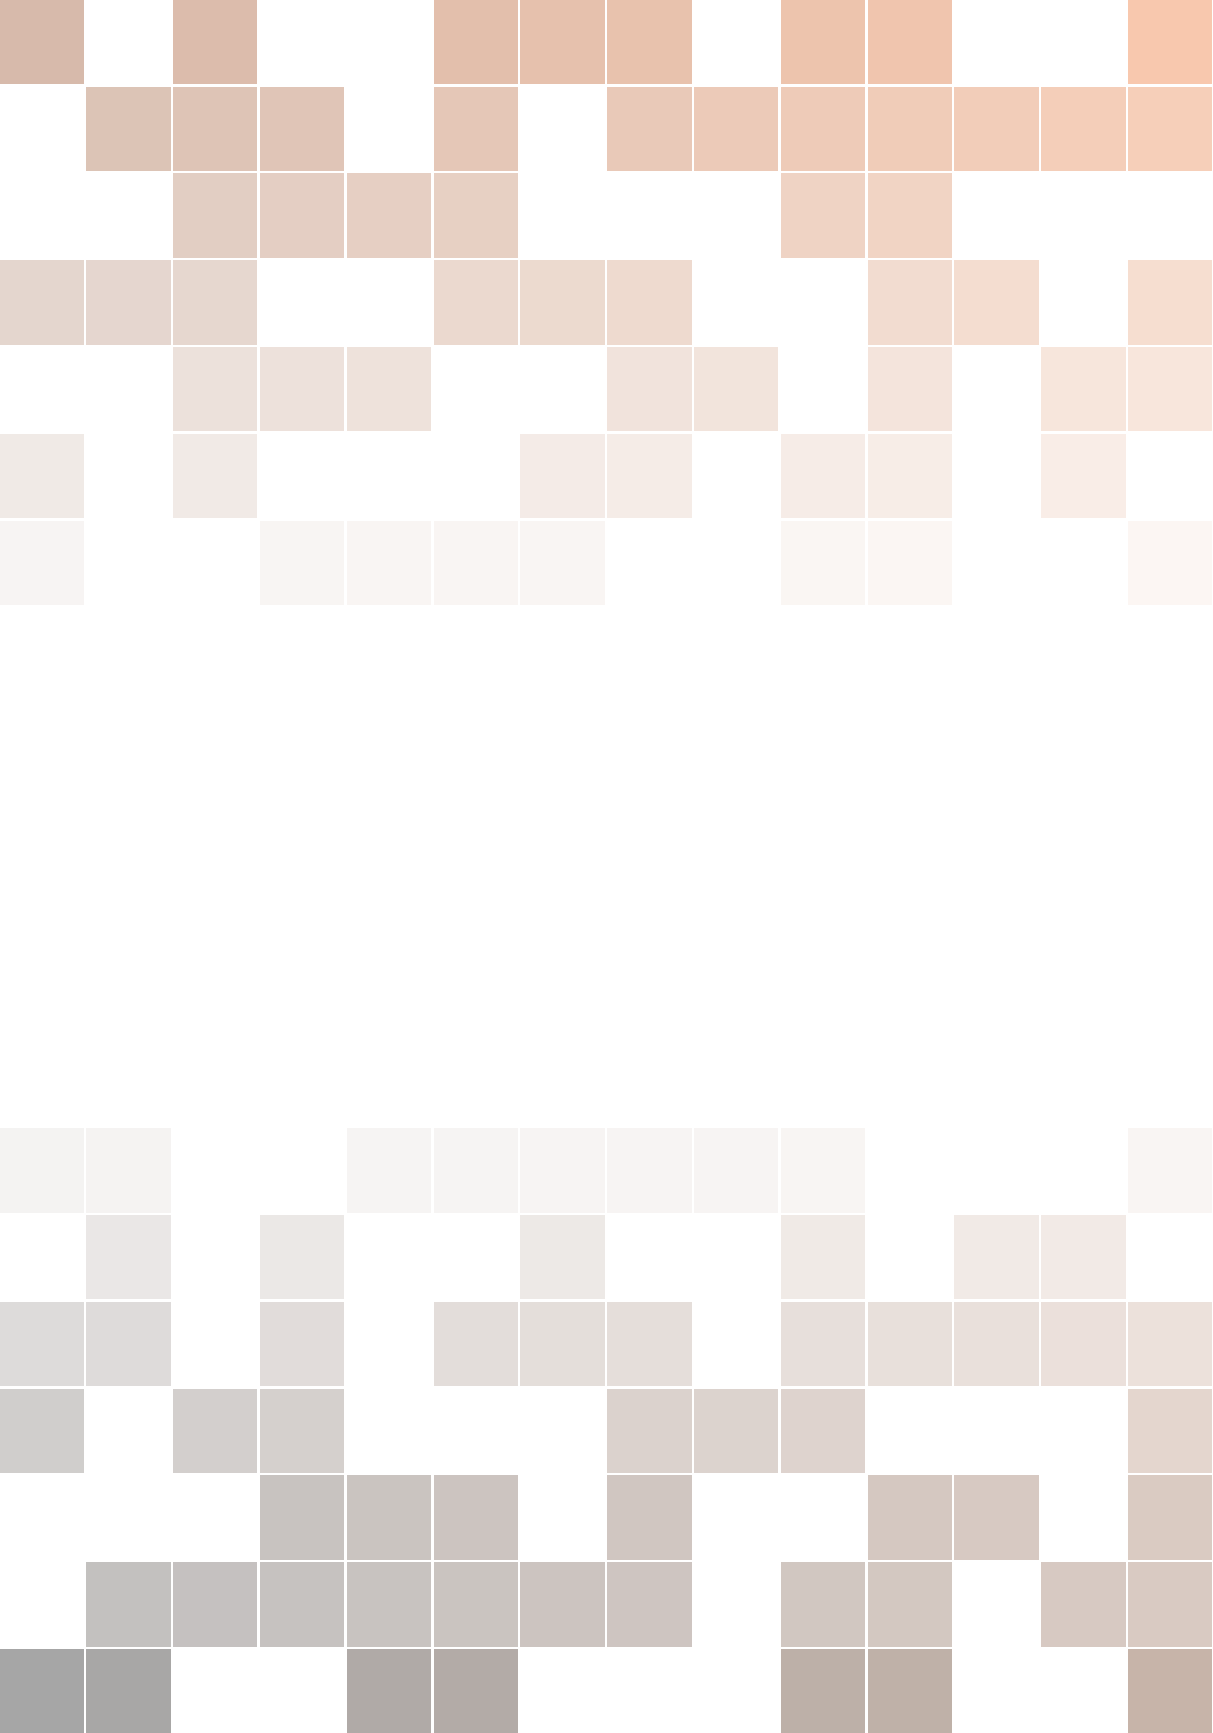
\includegraphics[width=\paperwidth]{background}};
\draw (current page.center) node [fill=ocre!30!white,fill opacity=0.6,text opacity=1,inner sep=1cm]{\Huge\centering\bfseries\sffamily\parbox[c][][t]{\paperwidth}{\centering Álgebra 1\\[15pt] % Book title
{\Large Notas de Aula 2/2017}\\[20pt] % Subtitle
{\huge Jos\'e Ant\^onio O. Freitas}\\
{\large \today}}}; % Author name

\end{tikzpicture}
\vfill
\endgroup

%----------------------------------------------------------------------------------------
%	COPYRIGHT PAGE
%----------------------------------------------------------------------------------------

\newpage
~\vfill
\thispagestyle{empty}

\noindent \ccbyncsa\ Este texto est\'a licenciado sob uma \textbf{Licen\c{c}a Creative Commons Atribui\c{c}\~ao-N\~aoComercial-CompartilhaIgual 3.0 Brasil} \href{http://creativecommons.org/licenses/by-nc-sa/3.0/br/deed.pt\_BR}{\textit{http://creativecommons.org/licenses/by-nc-sa/3.0/br/deed.pt\_BR}}\\ % Copyright notice

%----------------------------------------------------------------------------------------
%	TABLE OF CONTENTS
%----------------------------------------------------------------------------------------

\usechapterimagefalse % If you don't want to include a chapter image, use this to toggle images off - it can be enabled later with \usechapterimagetrue

\chapterimage{chapter_head_1.pdf} % Table of contents heading image

\pagestyle{empty} % No headers

\tableofcontents % Print the table of contents itself

\cleardoublepage % Forces the first chapter to start on an odd page so it's on the right

\pagestyle{fancy} % Print headers again


%!TEX program = xelatex
%!TEX root = Algebra_1.tex
%%Usar makeindex -s indexstyle.ist arquivo.idx no terminal para gerar o {\'\i}ndice remissivo agrupado por inicial
%%Ap\'os executar pdflatex arquivo
\chapter{Conceitos B\'asicos} % (fold)
\label{cha:conceitos_basicos}

\begin{definicao}
	Uma \textbf{proposi\c{c}\~ao} \'e todo conjunto de palavras ou s{\'\i}mbolos ao qual podemos atribuir um \textbf{valor l\'ogico}.
\end{definicao}

\begin{definicao}
	Diz-se que o \textbf{valor l\'ogico} de uma proposi\c{c}\~ao \'e ``verdade'' (V) se a proposi\c{c}\~ao \'e verdadeira ou ``falsidade'' (F) se a proposi\c{c}\~ao \'e falsa.
\end{definicao}

\begin{exemplos}
	Julgue se as seguintes sentenças são ou não proposições:
	\begin{enumerate}[label={\arabic*})]
		\item Todo número primo é ímpar.
		Essa setença é uma proposição de valor lógico "Falsidade."
		\item $x^2 + y^2 \ge 0$ para todos $x$, $y \in \real$.
		Esse setença é uma proposição de valor lógico "Verdade".
		\item Amanhã irá chover.
		Essa sentença não é uma proposição. Não é possível atribuir um valor lógico a ela.
	\end{enumerate}

\end{exemplos}

\section{Princ{\'\i}pio da n\~ao contradi\c{c}\~ao e do terceiro exclu{\'\i}do} % (fold)
\label{sec:principio_da_nao_contradicao_e_do_3}
\begin{enumerate}[label={\roman*})]
	\item Uma proposi\c{c}\~ao n\~ao pode ser verdadeira e falsa ao mesmo tempo.
	\item Toda proposi\c{c}\~ao ou \'e verdadeira ou \'e falsa, isto \'e, verifica-se sempre um destes casos e nunca um terceiro.
\end{enumerate}

Assim esses princ{\'\i}pios afirmam que:
\begin{center}
	``Toda proposi\c{c}\~ao tem um, e um s\'o, dos valores l\'ogicos \textbf{verdade} ou \textbf{falsidade}.''
\end{center}

De modo geral vamos trabalhar com proposi\c{c}\~oes da forma:
\begin{enumerate}[label={\roman*})]
	\item Se $\mathcal{H}$, ent\~ao $\mathcal{T}$.

	Aqui $\mathcal{H}$ \'e chamado de hip\'otese e $\mathcal{T}$ de tese. Neste tipo de proposi\c{c}\~ao iremos admitir que $\mathcal{H}$ \'e uma verdade e precisaremos provar que $\mathcal{T}$ \'e verdade. Ou seja precisamos construir um argumento que justifique $\mathcal{T}$ ser verdadeira \`a partir do fato de $\mathcal{H}$ ser verdadeira.

	\item $\mathcal{H}$ se, e somente se, $\mathcal{T}$ ou $\mathcal{H}$ se, e s\'o se, $\mathcal{T}$.

	Esse tipo de proposi\c{c}\~ao ser\'a decomposta em duas proposi\c{c}\~oes no formato anterior. Isto \'e:
	\begin{enumerate}[label={\alph*})]
		\item Se $\mathcal{H}$, ent\~ao $\mathcal{T}$.
		\item Se $\mathcal{T}$, ent\~ao $\mathcal{H}$.
	\end{enumerate}

	No primeiro caso admitimos $\mathcal{H}$ verdadeira e provamos que $\mathcal{T}$ tamb\'em \'e verdadeira e no segundo caso admitimos que $\mathcal{T}$ \'e verdadeira e provamos que $\mathcal{H}$ \'e verdadeira.
\end{enumerate}
% section pr{\'\i}ncipio_da_n\~ao_contradi\c{c}\~ao_e_do_3 (end)

% chapter conceitos_b\'asicos (end)

\chapter{No{\c c}{\~o}es de Teoria de Conjuntos}
\section{Conceitos b{\'a}sicos}

Um conjunto {\'e} uma ``cole{\c c}{\~a} o'' ou ``fam{\'\i}lia'' de elementos.

Usaremos letras mai{\'u}sculas do alfabeto para denotar os conjuntos e denotaremos elementos de um dado conjunto por letras min{\'u}sculas do alfabeto.

Dado um conjunto $A$, para indicar o fato de que $x$ {\'e} um elemento de $A$, escrevemos:
\[
x \in A.
\]

Para dizer que um elemento $x$ n{\~a}o pertence ao conjunto $A$, escrevemos:
\[
x \notin A.
\]

Um conjunto sem elementos {\'e} chamado de \textbf{conjunto vazio}. Tal conjunto {\'e} denotado por $\emptyset$.

Dado um conjunto $A$ e $x$ um elemento, ocorre sempre o uma das seguintes situa\c{c}\~oes:
\[
x \in A \mbox{ ou } x \notin A.
\]

Al{\'e}m disso, para dois elementos $x$, $y \in A$, ocorre exatamente uma das seguinte situa\c{c}\~oes:
\[
x = y \mbox{ ou } x \neq y.
\]

\section{Descri{\c c}{\~a}o de um conjunto}

Um conjunto $A$ pode ser dado pela simples listagem dos seus elementos, como por exemplo:
\begin{align*}
	A= \{1,2,3,4,5\}\\
	B = \{verdade, falso\}.
\end{align*}

Um conjunto tamb{\'e}m pode ser dado pela descri{\c c}{\~a}o das propriedades dos seus elementos, como por exemplo:
\[
A = \{n \mid n \mbox{ \'e m{\'u}ltiplo de } 2\} = \{2,4,6,...\}.
\]

\section{Alguns conjuntos importantes}
\begin{enumerate}[label={\arabic*})]
	\item $\n = \{0,1,2,3,...\}$ o conjunto do n{\'u}meros naturais.
	\item $\z = \{...,-2,-1,0,1,2,...\}$ o conjunto dos n{\'u}meros inteiros.
	\item $\n_0 = \{0,1,2,3,...\}$ o conjunto dos n{\'u}meros inteiros n{\~a}o negativos.
	\item $\real $ o conjunto dos n{\'u}meros reais.
	\item $\real^*$ o conjunto dos n{\'u}meros reais n{\~a}o nulos.
	\item $\rac = \left\{\dfrac{p}{q} \mid p,q \in \z, q \neq 0 \right\}$ o conjunto dos n{\'u}meros racionais.
\end{enumerate}

\section{Propriedades dos conjuntos}

\begin{definicao}
	Dados dois conjuntos $A$ e $B$, dizemos que $A$ e $B$ s{\~a}o \textbf{iguais} se, e somente se, eles t{\^e}m os mesmos elementos. Ou seja, para todo $x \in A$ temos que $x \in B$ e para todo $y \in B$ temos $y \in A$.
\end{definicao}

Se $A$ e $B$ s{\~a}o iguais, escrevemos $A = B$
\begin{align*}
	\{1,2,3,4\} &= \{3,2,1,4\}\\
	\{1,2,3\} &\ne \{2,3\} 
\end{align*}
	
\begin{definicao}
	Se $A$ e $B$ s{\~a}o dois conjuntos, dizemos que $A$ {\'e} um \textbf{subconjunto} de $B$ ou que $A$ \textbf{est\'a contido} em $B$ ou que $B$ \textbf{cont\'em} $A$ se todo elemento de $A$ for elemento de $B$. Ou seja, se para todo elemento $x \in A$, temos $x \in B$. Nesse caso, escrevemos $A \subseteq B$ ou $B \supseteq A$.
\end{definicao}


Caso $A$ seja um subconjunto de $B$ mas n{\~a}o {\'e} igual a $B$, escrevemos:
\[
A \subsetneq B.
\]

Nesse caso, dizemos que $A$ {\'e} um \textbf{subconjunto pr{\'o}prio} de $B$.

Para dizer que $A$ n{\~a}o est{\'a} contido em $B$, escrevemos $A \nsubseteq B$

Usando a defini\c{c}\~ao de contin\^encia de conjuntos podemos definir igualdade de conjuntos da seguinte forma:
\begin{center}
	\textbf{dois conjuntos $A$ e $B$ s\~ao iguais se, e somente se, $A \subseteq B$ e $B \subseteq A$}.
\end{center}

Ou seja,
\begin{center}
	\textbf{se $A = B$ ent{\~a}o $A \subseteq B$ e $B \subseteq A$}.
\end{center}

Além disso,
\begin{center}
	\textbf{se $A \subseteq B$ e $B \subseteq A$, ent{\~a}o $A = B$}.
\end{center}

Quando $A$ e $B$ n{\~a}o s{\~a}o iguais, escrevemos $A \neq B$. Para que $A \neq B$ devemos ter $A \nsubseteq B$ ou $B \nsubseteq A$. Isto é, precisamos encontrar algum elemento $x \in A$ tal que $x \notin B$ ou então encontrar $y \in B$ tal que $y \notin A$.

\begin{proposicao}
	Dados três conjuntos $A$, $B$ e $C$ temos:
	\begin{enumerate}[label={\roman*})]
		\item $A\subseteq A$ (Reflexividade)
		\item Se $A\subseteq B \mbox{ e } B\subseteq A$, ent{\~a}o $A=B$. (Antissimetria)
		\item Se $A\subseteq B$ e $B\subseteq C$, ent{\~a}o $A\subseteq C$. (Transitividade)
	\end{enumerate}
\end{proposicao}


Considere os seguintes conjuntos:
\begin{align*}
	A &= \{ n \in \n \mid n \mbox{ {\'e} m{\'u}ltiplo de } 2\} = \{2,4,6,...\}\\
	B &= \{n \in \n \mid n \mbox{ {\'e} m{\'u}ltiplo de } 3\} = \{3,6,9,...\}.
\end{align*}


Neste caso, $2 \in A$ e $2 \notin B$, logo $A \nsubseteq B$. Por outro lado, $3 \in B$ e $3 \notin A$ e com isso $B \nsubseteq A$. Portanto, dados dois conjuntos $A$ e $B$, nem sempre temos $A \subseteq B$ ou $B \subseteq A$.

\begin{proposicao} 
	Seja $A$ um conjunto. Ent{\~a}o $ \emptyset \subseteq A$.
\end{proposicao}
\begin{prova}
	Suponha que $\emptyset \nsubseteq A$. Logo existe $x \in \emptyset$ tal que $x \notin A$. Mas por defini{\c c}{\~a}o, o conjunto vazio n{\~a}o cont{\'e}m elementos. Logo a exist\^encia de $x \in \emptyset$ {\'e} uma contradi{\c c}{\~a}o. Tal contradi\c{c}\~ao surgiu por termos suposto que $\emptyset \nsubseteq A$. Portanto, $\emptyset \subseteq A$, como quer{\'\i}amos demonstrar.
\end{prova}

\section{Rela{\c c}{\~o}es entre conjuntos}

\begin{definicao}\label{intersecao_conjunto}
Sejam $A$ e $B$ dois conjuntos. Definimos a \textbf{intersec{\c c}{\~a}o} de $A$ e $B$ como sendo o conjunto $A \cap B$ cujos elementos pertencem ao conjunto $A$ e $B$ simultaneamente. Assim,
\[
A \cap B = \{x \mid x \in A\mbox{ e }  x \in B\}.
\]
\end{definicao}

\begin{exemplo}
	Sejam $A = \{1, 2, 3\}$, $B = \{2, 3, 4\}$ e $C = \{r, s, t\}$. Então
	\begin{align*}
		A \cap B &= \{2, 3\}\\
		A \cap C &= \emptyset.
	\end{align*}
\end{exemplo}

\begin{definicao}\label{unicao_conjuntos}
Sejam $A$ e $B$ dois conjuntos. Definimos a \textbf{uni{\~a}o} de $A$ com $B$ como sendo o conjunto $A \cup B$, cujos elementos pertencem ao conjunto $A$ ou ao conjunto $B$. Assim,
\[
A \cup B = \{x \mid x \in A \mbox{ ou } x \in B\}.
\]
\end{definicao}

\begin{exemplo}
	Sejam $A = \{1, 2, 3\}$, $B = \{2, 3, 4\}$ e $C = \{r, s, t\}$. Então
	\begin{align*}
		A \cup B &= \{1,2,3,4\}\\
		A \cup C &= \{1,2,3,r,s,t\}.
	\end{align*}
\end{exemplo}

\begin{proposicao} Sejam $A$ e $B$ dois conjuntos. Ent{\~a}o:
	\begin{enumerate}[label={\roman*})]
		\item $(A \cap B) \subseteq A$;
		\item $(A \cap B) \subseteq B$;
		\item $A \subseteq A \cup B$;
		\item $B \subseteq A \cup B$.
	\end{enumerate}
\end{proposicao}
\begin{prova}
	Para provar a primeira afirmação seja $x \in A \cap B$ um elemento qualquer. Da defini\c{c}\~ao de interse\c{c}\~ao de conjuntos, Definição \ref{intersecao_conjunto}, temos $x \in A$ e $x \in B$. Assim podemos afirmar com certeza que $x \in A$. Logo todo elemente de $A \cap B$ também está em $A$, ou seja, $A \cap B \subseteq A$. De modo análogo prova-se a segunda afirmação sobre interseção.

	Para a terceira afirmação, seja $x \in A$. Da definição de união de conjuntos, Definição \ref{unicao_conjuntos}, segue que $x \in A \cup B$. Logo todo elemento de $A$ também está em $A \cup B$, ou seja, $A \subseteq (A \cup B)$. De modo análogo prova-se a quarta afirmação.
\end{prova}

O conceito de uni{\~a}o ($ \cup $) e intersec{\c c}{\~a}o ($ \cap $) pode ser estendido para mais de dois conjuntos.

\begin{definicao}
Sejam $A_{1}$, \dots, $A_{n}$ conjuntos. Ent{\~a}o
\[
A_{1} \cup A_{2} \cup \cdots \cup A_{n}= \displaystyle\bigcup_{k=1}^n A_{k}
\]
{\'e} o conjunto dos elementos $x$ tais que $x$ pertence a pelo menos um dos conjuntos $A_{1}$, \dots, $A_{n}$. Agora,
\[
A_{1} \cap \cdots \cap A_{n} = \displaystyle\bigcap_{k=1}^{n}A_{k}
\]
{\'e} o conjunto dos elementos $x$ que pertencem a todos os conjuntos $A_{1}$, \dots, $A_{n}$ simultaneamente.
\end{definicao}

\begin{definicao}
	Sejam $A$ e $B$ conjuntos. Se $A \cap B = \emptyset$, dizemos que $A$ e $B$ s{\~a}o \textbf{conjuntos disjuntos}.	
\end{definicao}


Sejam $A$ e $B$ conjuntos tais que $C = A \cup B$ e $A \cap B = \emptyset$. Neste caso dizemos que $C$ {\'e} uma \textbf{uni{\~a}o disjunta} de $A$ e $B$. Denotamos tal fato por
\[
C = A \sqcup B.
\]

\begin{proposicao} Sejam $A,\ B$ e $C$ tr{\^e}s conjuntos, ent{\~a}o:
	\begin{enumerate}[label={\roman*})]
		\item $A\cap(B\cup C)=(A\cap B)\cup(A\cap C)$
		\item $A\cup(B\cap C)=(A\cup B)\cap(A\cup C)$
	\end{enumerate}
\end{proposicao}
\begin{prova}
	\begin{enumerate}[label={\roman*})]
		\item Precisamos mostrar que
		\begin{enumerate}[label={\roman*})]
			\item $A\cap(B\cup C)\subseteq(A\cap B)\cup(A\cap C)$;\label{intersecao_unicao_1}
			\item $(A\cap B)\cup(A\cap C)\subseteq A\cap(B\cup C).$\label{intersecao_unicao_2}
		\end{enumerate}

		Para provar \ref{intersecao_unicao_1} seja $x\in A \cap (B \cup C)$. Logo $x\in A$ e $x\in B\cup C$. Agora, de $x\in B\cup C$, segue que $x\in B$ ou $x\in C$. Suponha que $x\in B$. Como $x\in A$ e $x \in B$, ent\~ao $x\in A\cap B$. Assim, $x\in(A\cap B)\cup(A\cap C)$, ou seja, $A\cap(B\cup C)\subseteq(A\cap B)\cup(A\cap C)$. Por outro lado, se $x\in C$, como $x\in A$, ent{\~a}o $x\in A\cap C$ e da{\'\i} $x\in(A\cap B)\cup(A\cap C)$, logo $A\cap(B\cup C)\subseteq(A\cap B)\cup(A\cap C)$.

		Portanto,
		\[
			A\cap(B\cup C)\subseteq(A\cap B)\cup(A\cap C).
		\]

		Agora para provar \ref{intersecao_unicao_2}, seja $x\in(A\cap B)\cup(A\cap C)$. Da{\'\i}, $x\in A\cap B$ ou $x\in A\cap C$. Suponha que $x\in A\cap B$. Assim, $x\in A$ e $x\in B$. Como $x\in B$, segue que $x\in B\cup C$ e ent{\~a}o $x\in A\cap(B\cup C)$, ou seja, $(A\cap B)\cup(A\cap C)\subseteq A\cap(B\cup C)$. Agora, suponha que $x\in A\cap C$. Com isso $x\in A$ e $x\in C$. Desse modo, $x\in B\cup C$ e ent{\~a}o $x\in A\cap(B\cup C)$ e da{\'\i}
		\[
			(A\cap B)\cup(A\cap C)\subseteq A\cap(B\cup C).
		\]

		Portanto
		\[
			A\cap(B\cup C)=(A\cap B)\cup(A\cap C),
		\]
		como quer{\'\i}amos.
		\item An\'aloga ao caso anterior.
	\end{enumerate}
\end{prova}

\begin{definicao}
	Dados dois conjuntos $A$ e $B$, definimos a \textbf{diferen{\c c}a} dos conjuntos $A$ e $B$, denotada por $A-B$ ou $A\backslash B$ como sendo o conjunto
	\[
		A - B = \{x \mid x \in A \mbox{ e } x \notin B\}.
	\]
\end{definicao}

\begin{exemplos}
	\begin{enumerate}[label={\arabic*})]
		\item Se $A=\{1,2,3,5,4\}$, $B=\{2,3,6,8\}$, então
		\begin{align*}
			A - B &= \{1,4,5\}\\
			B - A &=\{6,8\}.
		\end{align*}
		\item Se $A=\{2,4,6,8,10,...\}$, $B=\{3,6,9,12,15,...\}$, então
		\begin{align*}
		 	A - B &= \{2,4,8,10,14,16,...\}\\
		 	B - A &= \{3,9,15,21,...\}
		 \end{align*}
	\end{enumerate}
	
\end{exemplos}

\begin{proposicao}
	Sejam $A$, $B$ e $C$ conjuntos n\~ao vazios. Ent\~ao
	\[(A \cup B) - C = (A - C) \cup (B - C).\]
\end{proposicao}
\begin{prova}
	Segue da defini\c{c}\~ao de diferen\c{c}a de conjuntos.
\end{prova}

\begin{definicao}
Dados dois conjuntos $A$ e $E$ tais que $A\subseteq E$, definimos o \textbf{complementar} de $A$ em $E$, denotado $A^C$ ou $C_E(A)$, como
\[
	C_E(A) = \{ x \in E \mid x \notin A \}.
\]
\end{definicao}

\begin{observacoes}
	\begin{enumerate}[label={\arabic*})]
		\item Se $A = E$, ent{\~a}o $C_A(A) = \{ x \in A \mid x \notin A \} = \emptyset$.
		\item $(A^C)^C = \{x \in E \mid x \notin A^C\} = \{ x \in E \mid x \in A \} = A$
	\end{enumerate}
	
\end{observacoes}

\begin{exemplo}
	Sejam $A = \{1,2,3,4\}$ e $E = \{1,2,3,5,4,0,8,9\}$. Primeiro note que $A \subseteq E$, daí
	\[
			A^C = C_E(A) = \{0,5,8,9\}.
	\]
\end{exemplo}

\begin{proposicao}
	Sejam $A$, $B$ e $E$ conjuntos. Se $A\subseteq B\subseteq E$, ent{\~a}o $C_E(B)\subseteq C_E(A)$.
\end{proposicao}
\begin{prova}
	Seja $x \in C_E(B)$. Assim $x\notin B$ e como $A \subseteq B$, ent\~ao $x \notin A$. Da{\'\i} por defini\c{c}\~ao $x\in C_E(A)$, ou seja, $C_E(B) \subseteq C_E(A)$.
\end{prova}

\begin{proposicao} Sejam $A$, $B$ e $E$ tr{\^e}s conjunto tais que $A\subseteq E$ e $B\subseteq E$. Ent{\~a}o:
\begin{enumerate}[label={\roman*})]
	\item $(A\cup B)^C = A^C\cap B^C$
	\item $(A\cap B)^C = A^C\cup B^C$
\end{enumerate}
\end{proposicao}
\begin{prova}
	\begin{enumerate}[label={\roman*})]
		\item Seja $x \in (A\cup B)^C$. Logo $x\notin A\cup B$, assim $x\notin A$ e $x\notin B$. Da{\'\i}, $x\in A^C$ e $x\in B^C$, isto {\'e}, $x\in A^C\cap B^C$. Desse modo,
		\begin{equation}\label{complementar_uniao-1}
			(A\cup B)^C \subseteq A^C\cap B^C.
		\end{equation}

		Por outro lado, se $x\in A^C\cap B^C$, ent{\~a}o $x\in A^C$ e $x\in B^C$. Com isso, $x\notin A$ e $x\notin B$, ou seja, $x\notin A\cup B$, logo $x\in (A\cup B)^C$. Desse modo
		\begin{equation}\label{complementar_uniao-2}
			A^C\cap B^C\subseteq(A\cup B)^C.
		\end{equation}

		Portanto, de \eqref{complementar_uniao-1} e \eqref{complementar_uniao-2} temos
		\[
			(A\cup B)^C = A^C\cap B^C.
		\]

		\item Seja $x \in (A\cap B)^C$. Logo $x\notin A\cap B$, assim $x\notin A$ ou $x\notin B$. Ent\~ao $x\in A^C$ ou $x\in B^C$, isto {\'e}, $x\in A^C\cup B^C$. Desse modo,
		\begin{equation}\label{complementar_intersecao-1}
			(A\cap B)^C \subseteq A^C\cup B^C.
		\end{equation}

		Por outro lado, se $x\in A^C\cup B^C$, ent{\~a}o $x\in A^C$ ou $x\in B^C$. Da{\'\i}, $x\notin A$ ou $x\notin B$, ou seja, $x\notin A\cap B$, logo $x\in (A\cap B)^C$. Desse modo
		\begin{equation}\label{complementar_intersecao-2}
			A^C\cup B^C\subseteq(A\cap B)^C.
		\end{equation}

		Portanto, de \eqref{complementar_intersecao-1} e \eqref{complementar_intersecao-2} temos
		\[
			(A\cap B)^C = A^C\cup B^C.
		\]
	\end{enumerate}
\end{prova}

\begin{definicao}
	Dados dois conjuntos $A$ e $B$, definimos o \textbf{produto cartesiano} de $A$ por $B$ como sendo o conjunto
	\[
		A \times B = \{(x,y) \mid x\in A, y\in B\}.
	\]
\end{definicao}

Dados $(x,y)$, $(z,t) \in A\times B$, temos
\begin{center}
	\textbf{$(x,y) = (z,t)$ se, e somente se, $x = z$ e $y = t$}.
\end{center}

\begin{exemplo}\label{exemplo_produto_cartesiano}
	Sejam $A = \{1,2\}$ e $B = \{3,4\}$. Então
	\begin{align*}
		A \times B &= \{(1,3), (1,4), (2,3), (2,4)\}\\
		B \times A &= \{(3,1), (3,2), (4,1), (4,2)\}
\end{align*}
\end{exemplo}

\begin{observacao}
	Do Exemplo \eqref{exemplo_produto_cartesiano} vemos que em geral $A \times B \neq B\times A$.
\end{observacao}

\begin{definicao}
	Para qualquer conjunto $A$, indicamos por $\mathcal{P}(A)$ o conjunto
	\[
		\mathcal{P}(A) = \{ X \mid X\subseteq A\}
	\]
	que \'e chamado de \textbf{conjunto das partes} de $A$.
\end{definicao}

Os elementos desse conjunto s{\~a}o todos os subconjuntos de $A$. Dizer que $Y\in \mathcal{P}(A)$ significa que $Y \subseteq A$. Particularmente, temos $\emptyset\in \mathcal{P}(A)$ e $A\in \mathcal{P}(A)$.

\begin{exemplos}
	\begin{enumerate}[label={\arabic*})]
		\item $A = \emptyset$, $\mathcal{P}(A) = \{\emptyset\}$;
		\item $B = \{x\}$, $\mathcal{P}(B) = \{\emptyset, \{x\}\}$;
		\item $C = \{a,b,c\}$, $\mathcal{P}(C)=\{\emptyset, \{a\}, \{b\},\{c\},\{a,b\},\{a,c\},\{b,c\},C\}$;
		\item $D=\real$, $\mathcal{P}(D)=\{X\mid X \subseteq \real\}$, por exemplo $\rac\in \mathcal{P}(D)$.
	\end{enumerate}	
\end{exemplos}
%!TEX program = xelatex
%!TEX root = Algebra1.tex
%%Usar makeindex -s indexstyle.ist arquivo.idx no terminal para gerar o {\'\i}ndice remissivo agrupado por inicial
%%Ap\'os executar pdflatex arquivo
\cleardoublepage
\phantomsection
\addcontentsline{toc}{chapter}{Bibliografia}
\renewcommand{\bibname}{Bibliografia}

\begin{thebibliography}{99}
\bibitem{HI} H.H. Domingues, G.Iezzi: \textit{{\'A}lgebra Moderna}, 2ª Ed., Atual, 1982
\bibitem{Shok} S. Shokranian: \textit{{\'A}lgebra 1}, Ci{\^e}ncia Moderna, 2010
\bibitem{AG} Adilson Gon{\c c}alves: \textit{Introdu{\c c}{\~a}o {\`a} {\'A}lgebra}, 5ª Ed., IMPA, 2003
\bibitem{Birk} G. Birkhoff, S. MacLane: \textit{{\'A}lgebra Moderna B{\'a}sica}, 4ª Ed., Guanabara Dois, 1980
\bibitem{Filho} E. A. Filho: \textit{Inicia{\c c}{\~a}o {\`a} L{\'o}gica Matem{\'a}tica}, Nobel, 2002
\end{thebibliography}
%----------------------------------------------------------------------------------------
%	BIBLIOGRAPHY
%----------------------------------------------------------------------------------------


%----------------------------------------------------------------------------------------
%	INDEX
%----------------------------------------------------------------------------------------

\cleardoublepage
\phantomsection
\setlength{\columnsep}{0.75cm}
\addcontentsline{toc}{chapter}{\textcolor{ocre}{Index}}
\printindex

%----------------------------------------------------------------------------------------

\end{document}
